%%=============================================================================
%% AutoKeras
%%=============================================================================

\chapter{AutoKeras}
\label{ch:autokeras}

In dit hoofdstuk wordt het volledige AutoKeras proces uitgelegd. Dit door belangrijke stukken code te nemen en expliciet toe te lichten welke keuzes gemaakt zijn en waarom. Ook \textit{performance metrics} worden hier verzameld en vergeleken. Het model is met verschillende parameter configuraties getraind. Elke variant blijft wel hetzelfde code skelet gebruiken.

De ontwikkeling is volledig in \textit{Jupyter notebooks}\footnote{\url{https://jupyter.org/}} uitgewerkt. Om de code makkelijk lokaal te gebruiken is \textit{Anaconda Navigator\footnote{\url{https://docs.anaconda.com/anaconda/navigator/}}} aangeraden, de meeste \textit{packages} worden standaard mee geïnstalleerd. De code bevindt zich ook in Appendix \ref{ch:app:autokeras} en kan online bekeken worden\footnote{\url{https://github.com/robbedec/bachproef-automl}}.

Het is ook mogelijk om de notebook in de cloud uit te voeren. De dataset (omgezet naar een numpy array) en de notebooks kunnen direct geüpload worden naar Google Colab of Kaggle. De gebruiker heeft dan voor een bepaalde duur gratis toegang tot grafische kaarten.

Volgende \textit{packages} moeten zelf geïnstalleerd worden:

\begin{itemize}
    \item tensorflow-gpu (2.1.0)
    \item autokeras (1.0.2)
    \item graphviz (0.13.2)
\end{itemize}

\section{Voorafgaand werk}
\label{sec:autokeras-before}

\subsection{GPU activatie}
\label{subsec:autokeras-gpu}

Het verloop van de code is ook hoe je een model van nul kan trainen. Er wordt gewerkt met een \textit{CUDA integrated GPU}. Tensorflow ondersteunt GPU acceleratie door middel van de CUDA Toolkit (cuDNN). Het installeren van de juiste drivers en toolkit zorgt er automatisch voor dat Tensorflow en subsequent ook Keras de grafische kaart herkennen en gebruiken om berekeningen mee te maken. Dit gedrag kan geverifieerd worden door enkele commando's uit te voeren in het \textit{notebook}. Als in de output een vermelding over de GPU staat mag u er vanuit gaan dat de die actief is. Meer informatie over de drivers / CUDA Toolkit en hoe ze geïnstalleerd moeten worden is te vinden op de site van NVIDIA\footnote{\url{https://developer.nvidia.com/hpc}}. Specifiek voor Tensorflow\footnote{\url{https://tensorflow.org/install/gpu}} is er een overkoepelende samenvatting die verschillende manieren beschrijft om de juiste \textit{tools} te installeren.

\bigskip

\begin{python}
from tensorflow.python.client import device_lib

def get_available_devices():
    local_device_protos = device_lib.list_local_devices()
    return [x.name for x in local_device_protos]
print(get_available_devices()) 
\end{python}

Een mogelijkse output kan er als volgt uitzien: ['/device:CPU:0', '/device:GPU:0'].

Op de cloud platformen moeten geen speciale drivers geïnstalleerd worden maar enkel een \textit{accelerator} geactiveerd zijn in het \textit{notebook}. Die kan geselecteerd worden in de instellingen van een \textit{notebook}.

\subsection{Data transformatie}
\label{subsec:autokeras-tranform}

De dataset bestaat deels uit een gelabelde afbeeldingen. Het bevat ook een verzameling ongelabelde afbeeldingen die tijdens de wedstrijd gebruikt werden als verificatie. In het kader van het onderzoek kunnen deze weggelaten worden en gaan we aan de slag met de gelabelde data. Elke afbeelding wordt genormaliseerd naar een standaard resolutie en omgezet naar een \textit{numpy array}\footnote{In de code is 'np' een verwijzing naar \textit{numpy}}. Dit zijn de kleurwaarden van elke pixel die samen een matrix vormen. Ook het label van de afbeelding is opgenomen in de matrix (0 = hond, 1 = kat). Momenteel staat alle data nog gegroepeerd volgens categorie. Voor de volgende stap is het belangrijk dat dit niet het geval is. Daarom wordt de matrix nog eens random gesorteerd.

Om consistentie tussen de experimenten te behouden wordt de matrix opgeslagen en bij een nieuwe configuratie terug ingeladen. De data transformatie wordt zo éénmaal uitgevoerd.

\bigskip

\begin{python}
def get_label(file):
    class_label = file.split('.')[0]
    if class_label == 'dog': label_vector = 0
    elif class_label == 'cat': label_vector = 1
    return label_vector
    
def get_data():
    data = []
    files = os.listdir(INPUT_PATH)
    
    for image in tqdm(files):
        label_vector = get_label(image)
        img = Image.open(INPUT_PATH + image).convert('L')
        img = img.resize((SIZE,SIZE))
    
        data.append([np.asarray(img),np.array(label_vector)])
        
    shuffle(data)
    return data

\end{python}

\section{Data preprocessing}
\label{sec:preprocessing-autokeras}

Een van de requirements is dat de \textit{preprocessing} voor de gebruiker gedaan wordt. Bij AutoKeras is dit niet 100\% het geval en moeten er zelf nog enkele zaken uitgevoerd worden. Zo moet de matrix die gemaakt is in sectie \ref{subsec:autokeras-tranform} opgedeeld worden in training en validatie datasets.

In \textit{data science} projecten wordt typisch x\_test en x\_train gebruikt om de \textit{features} van de afbeeldingen op te slaan, de matrix met pixel waarden. y\_test y\_train bevatten dan het bijhorend label. In de tweede stap wordt er dimensiereductie toegepast. De algoritmes houden geen rekening met kleuren dus die mogen we weglaten. De drie kleurendimensies (Rood, Groen, Blauw) worden omgezet naar één dimensie (grijswaarden). Deze conversie gebeurt in de laatste twee lijntjes van onderstaande code.

\bigskip

\begin{python}
x_train = np.array([data[0] for data in train], 'float32')
x_test = np.array([data[0] for data in test], 'float32')
y_train = [data[1] for data in train]
y_test = [data[1] for data in test]

x_train = np.array(x_train).reshape(-1,SIZE,SIZE,1)
x_test = np.array(x_test).reshape(-1,SIZE,SIZE,1)

x_train /= 255
x_test /= 255
\end{python}

\section{Model trainen en evalueren}
\label{sec:traineval-autokeras}

Na alle voorbereiding is het tijd om de \textit{classifier} in gang te steken. Hierbij moet enkel een naam (voor het uiteindelijke model) en het maximum aantal pogingen meegegeven worden. Op voorhand kan er niet ingesteld worden hoe lang er gezocht mag worden. Het is wel mogelijk dat het vroegtijdig beëindigd wordt (voor max. aantal pogingen bereikt is) omdat de \text{loss value} niet genoeg zakt over x-aantal iteraties.

Met de \pyth{clf.fit()} methode wordt het best passend model gekozen. Met de test dataset kan uiteindelijk de performantie van het model gemeten worden. \pyth{clf.evaluate()} geeft twee scores terug. Eerst de \textit{loss value}, het is een interpretatie die kijkt hoe goed het model scoort door training en test data te nemen. Let wel op dat de test dataset die wij definiëren enkel gebruikt wordt als \pyth{clf.evaluate()} uitgevoerd wordt. AutoKeras neemt van de trainings dataset standaard 20\% om te gebruiken als interne test data tijdens het trainen. De tweede waarde is het percentage van correct voorspelde afbeeldingen.

\bigskip

\begin{python}
clf = ak.ImageClassifier(max_trials=MAX_TRIES, name=OUTPUT_NAME)
clf.fit(x_train,y_train, verbose=2)

score = clf.evaluate(x_test, y_test)
\end{python}

Momenteel zit er een bug in het \textit{greedy} optimalisatie algoritme (dat standaard gebruikt wordt) van AutoKeras waardoor \textit{classifiers} met een max. aantal pogingen > 5 vroegtijdig beëindigd worden. Een voorlopige oplossing is om een de API van Automodel te gebruiken en zelf de instellingen te configureren. Achterliggend gebeurt dit ook als \pyth{ak.ImageClassifier()} geïnitialiseerd wordt. Als vervanging is er gekozen om \textit{random search} te gebruiken (zie sectie \ref{sec:hyperparameter-tuning}).

\bigskip

\begin{python}
clf = ak.AutoModel(
    inputs=[ak.ImageInput()], 
    outputs=[ak.ClassificationHead()], 
    tuner="random",
    max_trials=MAX_TRIES, 
    name=OUTPUT_NAME,
    overwrite=False
    )
    
clf.fit(x_train, y_train, verbose=2)
\end{python}

\section{Model visualisatie}
\label{sec:vis-autokeras}

\subsection{Confusion matrix}
\label{subsec:confusion-autokeras}

De \textit{confusion matrix} is waarschijnlijk één van de beste visualisaties om een inzicht in het model te krijgen. Voor elke categorie wordt het aantal juiste voorspellingen getoond maar ook het aantal afbeeldingen die aan de verkeerde categorie toegekend zijn. Een voorbeeld van een \textit{confusion matrix} is te vinden in afbeelding \ref{fig:confusion-matrices-autokeras}.

\bigskip

\begin{python}
plt.style.use('classic')
%matplotlib inline

mat = confusion_matrix(y_test, predictions.round())
labels = ['dog', 'cat']

sns.heatmap(mat.T, square=True, annot=True, fmt='d', cbar=False, xticklabels=labels, yticklabels=labels)
plt.xlabel('true category')
plt.ylabel('predicted category')
\end{python} 


\subsection{Verkeerde voorspellingen}
\label{subsec:wrong-predictions}

Om inzicht te krijgen in de verkeerde voorspellingen is het handig om die terug als afbeeldingen te tonen. Het kan een manier zijn om als persoon een patroon te vinden waartegen het model fouten maakt. Het zo gezegde ruis op de afbeeldingen. 

De eerste stap om voorspellingen op te splitsen is het interpreteren van de waarden. Zo krijg je bij een binair classificatieprobleem altijd een getal tussen 0 en 1 terug. Het kantelpunt is dan $\frac{1}{2}$, elke voorspelling die kleiner is wordt geclassificeerd als klasse 0 en alles groter als klasse 1. Om elke verkeerde voorspelling te zoeken kunnen we simpelweg het resultaat afronden en vergelijken met het bijhorend label.

\bigskip

\begin{python}
images = x_test.reshape(5000,64, 64)
incorrect_predictions = []

for i in range(0, len(predictions)):
    if predictions[i].round() != y_test[i]:
        incorrect_predictions.append(
            (i, images[i], predictions[i].round(4), y_test[i]))
\end{python}

In sectie \ref{sec:preprocessing-autokeras} zijn alle afbeeldingen omgezet naar grijswaarden. Als deze nu opnieuw geconverteerd worden zijn ze uiteraard zwart-wit foto's. Bij elke afbeelding wordt nog een legende gegenereerd. Zo is duidelijk te zien wat de index van de afbeelding is, wat de voorspelling van het model is (afgerond tot vier cijfers) en de werkelijke waarde.

\bigskip

\begin{python}
%matplotlib inline

figure, axes = plt.subplots(nrows=6, ncols=4, figsize=(16,16))

for axes, item in zip(axes.ravel(), incorrect_predictions):
    index, image, predicted, expected = item
    axes.imshow(image, cmap=plt.cm.gray_r)
    axes.set_xticks([])
    axes.set_yticks([])
    axes.set_title(f'index: {index}\np: {predicted}; e: {expected}')
    
plt.tight_layout()
\end{python}

Het resultaat van deze code is te zien in afbeelding \ref{fig:wrong-prediction-autokeras-5} en \ref{fig:wrong-prediction-autokeras-10}.

\subsection{Overzicht van de lagen}
\label{subsec:model-overview}

Het resultaat is een combinatie van Keras lagen (inputlagen, activatielagen, normalisatielagen...). Keras heeft een ingebouwde functie \pyth{model.summary()} die volgend resultaat oplevert:

\bigskip

\begin{python}
Model: "model"
_________________________________________________________________
Layer (type)                 Output Shape              Param #   
=================================================================
input_1 (InputLayer)         [(None, 64, 64, 1)]       0         
_________________________________________________________________
normalization (Normalization (None, 64, 64, 1)         3         
_________________________________________________________________
conv2d (Conv2D)              (None, 62, 62, 32)        320       
_________________________________________________________________
conv2d_1 (Conv2D)            (None, 60, 60, 64)        18496     
_________________________________________________________________
max_pooling2d (MaxPooling2D) (None, 30, 30, 64)        0         
_________________________________________________________________
dropout (Dropout)            (None, 30, 30, 64)        0         
_________________________________________________________________
flatten (Flatten)            (None, 57600)             0         
_________________________________________________________________
dropout_1 (Dropout)          (None, 57600)             0         
_________________________________________________________________
dense (Dense)                (None, 1)                 57601     
_________________________________________________________________
classification_head_1 (Sigmo (None, 1)                 0         
=================================================================
Total params: 76,420
Trainable params: 76,417
Non-trainable params: 3
_________________________________________________________________
\end{python}

Het overzicht kan ook geëxporteerd worden naar een afbeelding die beter geformatteerd is. De geëxporteerde afbeeldingen bevinden zich in Appendix \ref{ch:app:autokeras}.

\section{Resultaten}
\label{sec:results-autokeras}

Zoals eerder vermeld zijn er 2 modellen getraind met als enigste configuratieverschil, het maximum aantal pogingen. In andere woorden is dit het aantal verschillende Keras modellen dat aangemaakt mag worden. De resultaten van beide zijn samengevat in tabel \ref{table:autokeras-results}. 

Verder worden beide modellen vermeld als model A (max. 5 pogingen) en model B (max. 10 pogingen).

\begin{minipage}{\textwidth}
    De specificaties van het host systeem zijn:
    \begin{itemize}
        \item CPU: i7-7700HG
        \item GPU: Nvidia GeForce GTX 1050 Ti Max-Q
        \item RAM: 16GB
    \end{itemize}
\end{minipage}

\bigskip

\begin{table}[ht]
    \centering
    \begin{tabular}{c c c c c c} % centered columns (4 columns)
        \hline\hline %inserts double horizontal lines
        Max aantal pogingen & Accuracy & Loss & Trainingsduur & Aantal lagen \\ [0.5ex] % inserts table
        %heading
        \hline % inserts single horizontal line
        5   & 82.74\%   & 0.6383   & 2u    & 10 \\ 
        \hline %inserts single line
        10   & 81.37\%   & 0.7110   & 8u    & 10 \\ 
        \hline
    \end{tabular}
    \caption{Resultaten AutoKeras.}
    \label{table:autokeras-results}
\end{table}

\begin{figure}[b!]
    \centering
    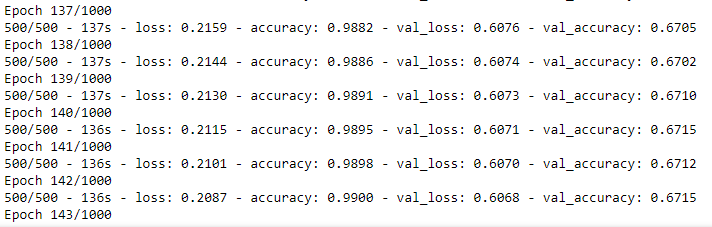
\includegraphics[width=\linewidth]{img/autokeras-overfit.png}
    \caption{Het model expres \textit{overfitten} in het kader van \textit{ensemble construction}.}
    \label{fig:autokeras-overfit}
\end{figure}

Wat meteen opvalt is dat een hoger aantal pogingen geen zekerheid is op betere prestaties. Zo wordt enkel de mogelijkheid gegeven op een uitgebreidere exploratie van de zoekruimte. Zo kan het algoritme bijvoorbeeld een extreem \textit{overfitted} model trainen in de hoop om die later te combineren met een andere om een beter resultaat te bekomen, een toepassing van \textit{ensemble construction} (zie sectie \ref{subsec:ensemble-construction}). Afbeelding \ref{fig:autokeras-overfit} komt rechtstreeks uit de output van model B en is niet te vinden in model A.

\begin{figure}[b!]
    \begin{subfigure}{0.5\textwidth}
        \centering
        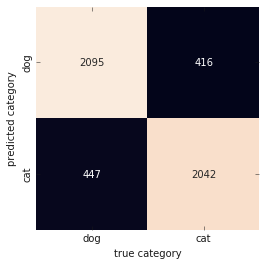
\includegraphics[width=0.8\linewidth]{img/autokeras-5-confusion.png}
        \caption{Max. pogingen = 5}
        \label{fig:confusion-autokeras-5}
    \end{subfigure}
    \begin{subfigure}{0.5\textwidth}
        \centering
        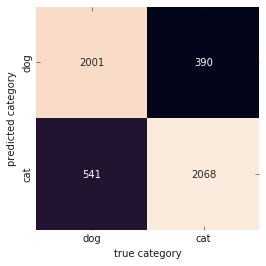
\includegraphics[width=0.8\linewidth]{img/autokeras-10-confusion.png}
        \caption{Max. pogingen = 10}
        \label{fig:confusion-autokeras-10}
    \end{subfigure}
    \caption{Overzicht confusion matrices}
    \label{fig:confusion-matrices-autokeras}
\end{figure}

\begin{minipage}{\textwidth}
De \textit{confusion matrices} in afbeelding \ref{fig:confusion-matrices-autokeras} tonen dat verspreiding van voorspellingen in beide gevallen redelijk overeen komt. Er is te zien dat model B meer aanleunt (en dus meer fouten maakt in die categorie) om kat te voorspellen dan hond, iets dat in model A in evenwicht is.
\end{minipage}

\begin{figure}
    \centering
    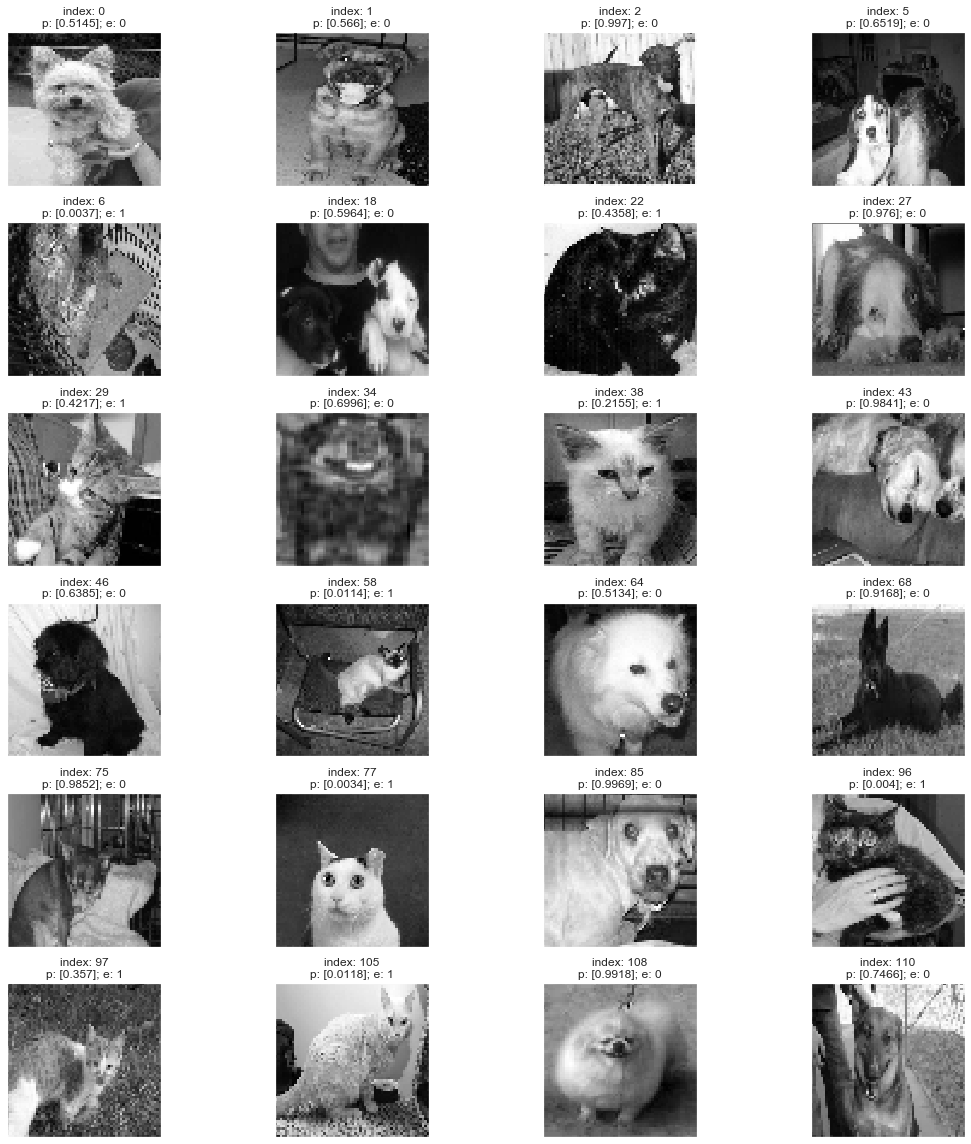
\includegraphics[width=\linewidth]{img/autokeras-5-wrong-images.png}
    \caption{Verkeerd voorspelde afbeeldingen van model A.}
    \label{fig:wrong-prediction-autokeras-5}
\end{figure}

\begin{figure}
    \centering
    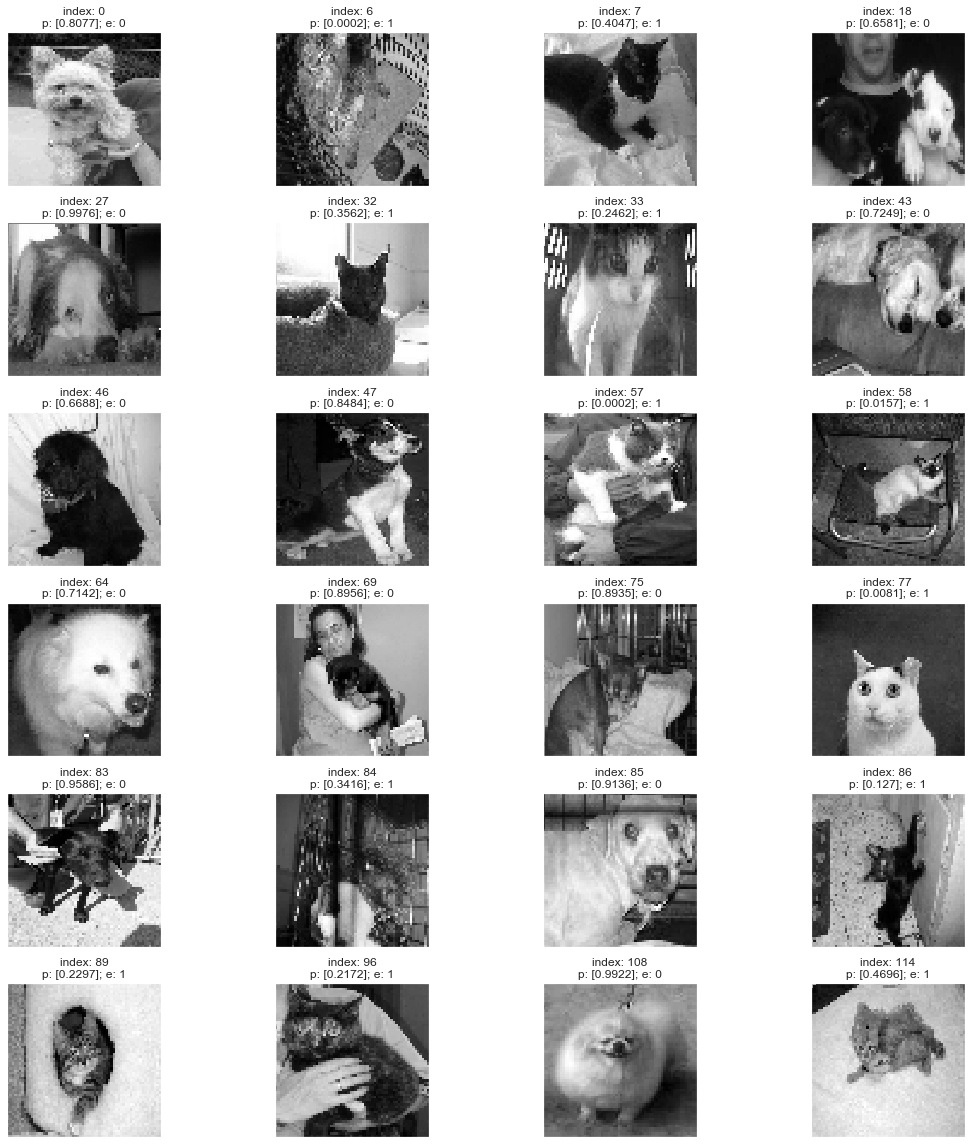
\includegraphics[width=\linewidth]{img/autokeras-10-wrong-images.png}
    \caption{Verkeerd voorspelde afbeeldingen van model B.}
    \label{fig:wrong-prediction-autokeras-10}
\end{figure}

Van beide modellen zijn 24 verkeerd voorspelde afbeeldingen gevisualiseerd (zie Figuren \ref{fig:wrong-prediction-autokeras-5} en \ref{fig:wrong-prediction-autokeras-10}). Bij sommige afbeelding kan duidelijk afgeleid worden wat de oorzaak is, mensen of andere onbekende objecten op de foto's. Andere zijn moeilijker te verklaren. Voor nu kan er besloten worden dat het model waarschijnlijk moeite heeft met de gespitste oren. Een typisch kenmerk van katten maar het komt soms ook voor bij honden. Maar ook het feit dat soms het volledige lichaam afgebeeld is en soms maar een deel van het hoofd.

Met een gemiddelde score van 82\% bekomen we een goed resultaat als er rekening gehouden wordt met de beperkte hoeveelheid \textit{data preprocessing}. Om dit op productie niveau te krijgen moet er wel meer moeite gedaan worden om de trainingsdataset beter te verwerken. AutoKeras is een exploratiemiddel, daarom zijn er voorlopig geen andere functies in de \textit{library} om het verwerken van de dataset te verbeteren. Handgemaakte modellen uit de competitie behalen scores tot 98\%\footnote{\url{https://www.kaggle.com/c/dogs-vs-cats/leaderboard}}.

Tijdens het trainingsproces heeft de aanwezigheid van een TPU geen invloed op de snelheid. Deze wordt gewoonweg niet gebruikt. Een TPU of \textit{tensor processing unit} is een schakeling van \textit{accelerators} die het proces vele malen sneller uitvoert. AutoKeras bied op dit moment geen ondersteuning om deze te gebruiken waardoor er teruggevallen wordt op de GPU's. De afwezigheid vormt wel een nadeel aangezien TPU's verder uitgroeien tot de nieuwe industrie standaard.

Voor een open-source library zit er zeker potentieel in voor de toekomst als u weet dat op een gelijkaardig niveau van \textit{preprocessing} en dezelfde dataset, een pre-release versie van AutoKeras slechts 67\% behaalde \autocite{Chopra2019}.

\section{Requirements}

\subsection{Functionele requirements}
\label{subsec:autokeras-fr}

\subsubsection{Implementatie van het procesmodel}
\label{sucsubsec:autokeras-fr-procesmodel}

Er is geen sprake van een volledige implementatie. Als open source project dient het in de eerste plaats als een onderzoeksproject. AutoKeras is simpelweg hun contributie aan de \textit{state of the art}. Niet commercieel onderzoek heeft weinig last van economische druk waardoor nieuwe \textit{features} soms lang op zich laten wachten. 

Bij AutoKeras moet \textit{data preprocessing} zelf uitgevoerd worden. De optimalisatiealgoritmen gaan zelf de belangrijke \textit{features} zoeken en selecteren. Dit houdt in dat de data getransformeerd moet worden (numpy array in de juiste dimensies), opgesplitst en aangepast volgens de intenties van de gebruiker vooraleer het gebruikt kan worden door \pyth{ImageClassifier()}.

\subsubsection{Beschikbare metrics}
\label{sucsubsec:autokeras-fr-metrics}

De output van het algoritme wordt geëxporteerd naar een gecompileerd Keras model, onderling gebruikt het ook Keras lagen. Dit wil zeggen dat alle mogelijke visualisaties van Keras perfect mogelijk zijn met de output. In het experiment gaat het dan vooral over \pyth{model.summary()} en gelijkaardige output die ons een inkijk in het resultaat geeft.

Omdat de ruwe resultaten ook beschikbaar zijn, is de gebruiker vrij om andere \textit{packages} te gebruiken. Zo kan met een lijst voorspellingen een \textit{confusion matrix} gemaakt worden aan de hand van de scikit-learn \textit{library}. De array van grijswaarden kan ook terug omgezet worden naar afbeeldingen om bijvoorbeeld, verkeerde voorspellingen te tonen. Alle verschillende mogelijkheden zijn enkel begrensd door het aantal beschikbare \textit{packages}.

Met de wiskundige formules kunnen ook allemaal verschillende statistieken berekend worden.

\subsubsection{Batch verwerking}
\label{sucsubsec:autokeras-fr-batch}

Voor een AutoKeras \textit{classifier} bestaat op de \pyth{ImageClassifier.fit()} methode een \textit{batch\_size} argument die dit kan manipuleren. Deze optie bepaalt hoeveel afbeeldingen er bij elke iteratie gepropageerd worden door het model. Door \textit{mini batches} te gebruiken moeten niet alle afbeeldingen op hetzelfde moment in het geheugen van de computer geladen worden. Onderliggend gebeuren er meer updates aan de \textit{gradient} die tot betere resultaten kunnen leiden.

\subsection{Niet-functionele requirements}
\label{subsec:autokeras-nfr} 

\subsubsection{Deployment}
\label{sucsubsec:autokeras-nfr-deployment}

De \textit{library} biedt geen mogelijkheden aan om een model te \textit{deployen}. Als gebruiker ben je zelf verantwoordelijk om de benodigde infrastructuur te voorzien. Ook zijn er mogelijks uitbreidingen nodig om de implementatie op productieniveau te krijgen. Meer informatie hierover in sectie \ref{sec:deployment}.

\subsubsection{Performantie}
\label{sucsubsec:autokeras-nfr-performantie}

Het uiteindelijke resultaat in ons experiment is bruikbaar. Met 83\% is de technologie op zich bewezen. Betere resultaten hangen sterk af van de hoeveelheid en kwaliteit van de \textit{data preprocessing}.

\subsubsection{Kostprijs}
\label{sucsubsec:autokeras-nfr-price}

Het gebruik van de \textit{library} zelf is volledig gratis. Ook voor het resultaat moet niet betaalt worden. Er moet zelf gekozen worden over welke investeringen gedaan worden in verband met de infrastructuur (aantal GPU's, kloksnelheid, elektriciteit ... ). Op zich kan een model getraind worden op een (gratis) online platform zoals Kaggle, of Google Colab. Om langere GPU tijden te verkrijgen kan een pro account aangeschaft worden.

\subsubsection{Verwerking}
\label{sucsubsec:autokeras-nfr-verwerking}

Omdat de meeste \textit{wrappers} geschreven zijn in Python, is het een goede keuze om er een eigen API mee te maken. Voor Flask zijn er online zeer veel \textit{tutorials} beschikbaar. Ook hierover is meer informatie te vinden in sectie \ref{sec:deployment}.